\documentclass[aspectratio=169]{beamer}

\usetheme{Madrid}
\usecolortheme{default}

\usepackage[utf8]{inputenc}
\usepackage{amsmath}
\usepackage{amsfonts}
\usepackage{amssymb}
\usepackage{graphicx}
\usepackage{qrcode}
\usepackage{booktabs}
\usepackage{tikz}
\usetikzlibrary{shapes,arrows,positioning,fit,calc,decorations.pathreplacing,backgrounds}
\usepackage{smartdiagram}
\usepackage{pgfplots}
\pgfplotsset{compat=1.18}
\usepackage{xcolor}

% --- Notes Setup ---
% SLIDES only (default): \setbeameroption{hide notes}
% SCRIPT only:           \setbeameroption{show only notes}
% Both on-screen:        \setbeameroption{show notes on second screen=right}
\usepackage{pgfpages}
\usepackage{multimedia}   % Beamer video embedding
\setbeameroption{hide notes}

% Shortcut macros for notes
\newcommand{\script}[1]{\note[item]{\textbf{Script:} #1}}
\newcommand{\qa}[2]{\note[item]{\textbf{Q:} \textit{#1} \\ \textbf{A:} #2}}

% --- Custom Colors ---
\definecolor{plantgreen}{RGB}{34, 139, 34}
\definecolor{herbired}{RGB}{180, 30, 30}
\definecolor{signalorange}{RGB}{220, 120, 0}
\definecolor{toxinpurple}{RGB}{100, 0, 150}
\definecolor{soilbrown}{RGB}{101, 67, 33}

% --- Title Info ---
\title[PlantProtectionSim]{\textit{A Visual Discrete Event-based Simulator for the\\Optimization of Plant Defense Strategies against Herbivores}}
\subtitle{Application of an Extended Tissue P System}
\author[B. Förster (Presenter)]{Lucas Dietrich \and \underline{Benjamin Förster} \and Peter Langendörfer \and Thomas Hinze}
\institute[BTU]{
    Hamburg University of Technology \and
    Brandenburg University of Technology \and
    Friedrich Schiller University Jena
}
\date{ICMC 2026 -- Seville (Spain)}

\begin{document}

% =====================================================================
% Slide 1: Title
% =====================================================================
\begin{frame}
    \titlepage
    \script{Welcome everyone. My name is Benjamin Förster. Today I'll present our research: a \textbf{visual discrete-event simulator} for plant defense strategies, built on \textbf{Extended Tissue P Systems}. We call it PlantProtectionSim.}
\end{frame}

% =====================================================================
% Slide 2: Biological Motivation
% =====================================================================
\begin{frame}{Biological Motivation: Plant Survival}
    \begin{columns}[T, onlytextwidth]
        \column{0.5\textwidth}
        \vspace{0.3cm}
        Plants face a fundamental constraint: \textbf{no mobility, no nervous system}.
        \vspace{0.3cm}
        \begin{itemize}
            \item \textbf{Constitutive:} Permanent, passive defense (thorns, bark, alkaloids). Low but constant energy drain.
            \item \textbf{Induced:} Triggered by attack. High-precision biochemical cascade.
            \item \textbf{Activated:} Chemically primed, latently deployed. Intermediate energy cost.
        \end{itemize}

        \column{0.5\textwidth}
        \vspace{0.2cm}
        \begin{center}
            \includegraphics[width=0.9\textwidth, keepaspectratio]{misc/lukas_simulator.png}

            \vspace{0.2cm}
            \parbox{0.9\textwidth}{\scriptsize \textbf{Visualisation:} Grid showing a spreading \textbf{VOC (Volatile Organic Compound)} signal. The expanding borders represent an airborne chemical warning emitted by an attacked plant, which primes neighboring plants for defense.}
        \end{center}
    \end{columns}
    \script{Plants face one ultimate constraint: no mobility, no nervous system. \textbf{Three defense layers} exist -- \textbf{Constitutive} (passive, always on), \textbf{Induced} (triggered on attack), and \textbf{Activated/Primed} (chemically warned in advance). Our simulator focuses on Induced and Activated dynamics. The image shows our grid when a VOC -- Volatile Organic Compound -- is emitted by an attacked plant and \textbf{spreads to prime its neighbors}.}
    \qa{Why not model constitutive defenses?}{They are static energy drains. Our goal is to study dynamic, event-based resource allocation and signaling, which yields far richer emergent behavior.}
    \qa{What does VOC stand for?}{Volatile Organic Compound -- gaseous chemicals emitted by plants to communicate stress or deter pests.}
\end{frame}

% =====================================================================
% Slide 3: The Optimization Problem
% =====================================================================
\begin{frame}{The Core Optimization Problem}
    \begin{columns}[T, onlytextwidth]
        \column{0.55\textwidth}
        Every plant has a \textbf{limited energy budget} $e$. Spending on defense reduces capacity for growth and reproduction.
        \vspace{0.3cm}
        \begin{itemize}
            \item \textbf{Goal:} Identify spatial configurations and defense trigger thresholds that maximize long-term survival.
            \item \textbf{Challenge:} The search space is vast -- 2 plant species $\times$ 2 herbivore species $\times$ 3 substances $\times$ continuous parameters.
            \item \textbf{Solution:} \textit{In-silico} simulation with the \texttt{PlantProtectionSim} tool.
        \end{itemize}

        \column{0.45\textwidth}
        \vspace{0.8cm}
        \begin{center}
        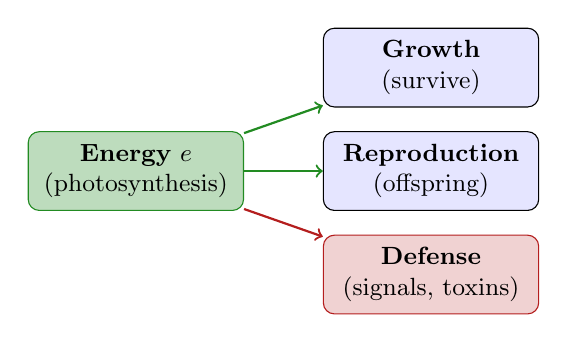
\begin{tikzpicture}[
            box/.style={rectangle, draw, rounded corners, fill=blue!10, text width=2.5cm, align=center, minimum height=1.0cm, font=\small}
        ]
            \node[box, fill=plantgreen!30, draw=plantgreen] (e) {\textbf{Energy $e$}\\(photosynthesis)};
            \node[box, right=1.0cm of e, fill=blue!10] (r) {\textbf{Reproduction}\\(offspring)};
            \node[box, above=0.3cm of r, fill=blue!10] (g) {\textbf{Growth}\\(survive)};
            \node[box, below=0.3cm of r, fill=herbired!20, draw=herbired] (d) {\textbf{Defense}\\(signals, toxins)};

            \draw[->, thick, plantgreen] (e) -- (g);
            \draw[->, thick, plantgreen] (e) -- (r);
            \draw[->, thick, herbired] (e) -- (d);
        \end{tikzpicture}
        \end{center}
    \end{columns}
    \script{Every plant has a \textbf{limited energy budget} -- photosynthesis yields energy which must be split between Growth, Reproduction, and Defense. Spend too much on defense and you are outcompeted. Too little and you get eaten. The \textbf{search space for optimal strategies is vast}: multiple species, continuous parameters, spatial dynamics. This makes analytical models insufficient -- \textbf{we need in-silico simulation}.}
    \qa{How is energy quantified?}{As a discrete abstract token $e$ produced each time step, representing net photosynthetic yield. It is consumed as currency by defense mechanisms.}
\end{frame}

% =====================================================================
% Slide 4: Communication Networks
% =====================================================================
\begin{frame}{Two Signaling Pathways}
    \begin{columns}[T, onlytextwidth]
        \column{0.5\textwidth}
        \textbf{Airborne (VOC) Signals}
        \begin{itemize}
            \item Gaseous molecules spread in concentric circles.
            \item Radius expands by 1 cell every \texttt{sendingSpeed} steps.
            \item Any plant within radius that is registered as a \texttt{receive} subscriber reacts.
        \end{itemize}
        \vspace{0.3cm}
        \begin{center}
        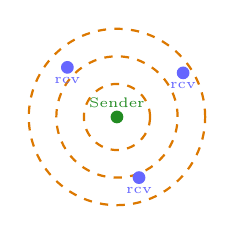
\begin{tikzpicture}[scale=0.7]
            \filldraw[plantgreen] (0,0) circle (3pt) node[above, font=\tiny]{Sender};
            \foreach \r in {0.6, 1.1, 1.6}{
                \draw[signalorange, dashed, thick] (0,0) circle (\r);
            }
            \foreach \x/\y in {1.2/0.8, -0.9/0.9, 0.4/-1.1}{
                \filldraw[blue!60] (\x,\y) circle (3pt) node[below, font=\tiny]{rcv};
            }
        \end{tikzpicture}
        \end{center}

        \column{0.5\textwidth}
        \textbf{Mycorrhizal (Symbiotic) Network}
        \begin{itemize}
            \item Underground fungal connections between adjacent plants.
            \item Targeted, edge-based: \texttt{SymbioticConnection(p1, p2)}.
            \item Requires Manhattan distance of 1 (direct neighbors only).
        \end{itemize}
        \vspace{0.3cm}
        \begin{center}
        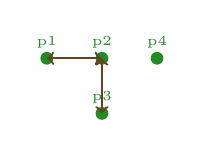
\begin{tikzpicture}[scale=0.7]
            \foreach \x/\y/\n in {0/0/p1, 1/0/p2, 1/-1/p3, 2/0/p4}{
                \filldraw[plantgreen] (\x,\y) circle (3pt) node[above, font=\tiny]{\n};
            }
            \draw[soilbrown, thick, <->] (0,0) -- (1,0);
            \draw[soilbrown, thick, <->] (1,0) -- (1,-1);
        \end{tikzpicture}
        \end{center}
    \end{columns}
    \script{We model two distinct biological signaling pathways. \textbf{Airborne VOCs spread radially} across the grid at a rate of \texttt{sendingSpeed} cells per step, allowing any subscribed plant within the radius to react. \textbf{Mycorrhizal signals} travel exclusively through \textbf{formal graph edges} -- strictly between adjacent plants (Manhattan distance of 1). Signals are only created by plants that actively detect an attack, meaning the herbivore cluster size on their cell has \textbf{exceeded a specific \texttt{triggerCombination} threshold}. Furthermore, emitting a signal is not free; the sending plant must \textbf{pay a predefined \texttt{energyCost}} from its internal energy token reserves, creating a realistic trade-off between communication and personal defense.}
    \qa{How is the signal object formally propagated in the Tissue P system?}{For VOCs, the signal object $s_i$ is placed into the environmental multiset and expands spatially. For mycorrhizal networks, $s_i$ uses symport rules along the specific structural edges defined in $E$ between adjacent plant membranes.}
\end{frame}

% =====================================================================
% Slide 5: Tissue P Systems
% =====================================================================
\begin{frame}{Formal Foundation: Tissue P Systems}
    \begin{columns}[T, onlytextwidth]
        \column{0.55\textwidth}
        \textbf{Why Tissue P Systems?}
        \begin{itemize}
            \item Designed for distributed computation across multiple membranes.
            \item Naturally encode \textbf{spatial topology} and \textbf{parallel rule application}.
            \item Every grid cell $V_{\mu,\nu}$ is an independent membrane with its own multiset.
        \end{itemize}
        \vspace{0.15cm}
        \centering
        {\small\begin{tabular}{@{}ll@{}}
            \toprule
            Biology & P System \\
            \midrule
            Grid cell & Membrane $V_{\mu,\nu}$ \\
            Plant state & State $q \in Q$ \\
            Chemicals & Object multiset $w$ \\
            Ecological events & Rules $r \in \mathcal{R}$ \\
            \bottomrule
        \end{tabular}}

        \column{0.45\textwidth}
        \vspace{-.5cm}
        \begin{center}
        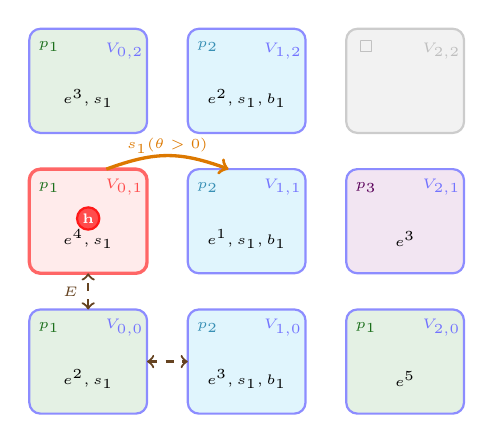
\begin{tikzpicture}[scale=1.15]
            % stepX=1.75, stepY=1.55, cell w=1.30, h=1.15
            % Fill colors encode species: p1=green, p2=cyan, p3=violet, empty=gray
            % Red border/fill on attacked cell (0,1)

            % === Row y=2 ===
            \draw[blue!45,thick,rounded corners=4pt,fill=plantgreen!12]
                (0,3.10) rectangle (1.30,4.25);
            \node[font=\tiny\bfseries,plantgreen!80!black] at (0.22,4.05) {$p_1$};
            \node[font=\tiny,blue!55] at (1.05,4.00) {$V_{0,2}$};
            \node[font=\tiny] at (0.65,3.48) {$e^3,s_1$};

            \draw[blue!45,thick,rounded corners=4pt,fill=cyan!12]
                (1.75,3.10) rectangle (3.05,4.25);
            \node[font=\tiny\bfseries,cyan!70!black] at (1.97,4.05) {$p_2$};
            \node[font=\tiny,blue!55] at (2.80,4.00) {$V_{1,2}$};
            \node[font=\tiny] at (2.40,3.48) {$e^2,s_1,b_1$};

            \draw[gray!40,thick,rounded corners=4pt,fill=gray!10]
                (3.50,3.10) rectangle (4.80,4.25);
            \node[font=\tiny\bfseries,gray!60] at (3.72,4.05) {$\square$};
            \node[font=\tiny,gray!50] at (4.55,4.00) {$V_{2,2}$};

            % === Row y=1 ===
            % Cell (0,1): ATTACKED — red border, herbivore marker
            \draw[red!60,very thick,rounded corners=4pt,fill=red!8]
                (0,1.55) rectangle (1.30,2.70);
            \node[font=\tiny\bfseries,plantgreen!80!black] at (0.22,2.50) {$p_1$};
            \node[font=\tiny,red!70] at (1.05,2.50) {$V_{0,1}$};
            \node[font=\tiny] at (0.65,1.93) {$e^4, s_1$};
            % Herbivore cluster dot
            \filldraw[red!70,draw=red!90,thick] (0.65,2.155) circle (3.5pt);
            \node[font=\tiny\bfseries,white] at (0.65,2.155) {h};

            \draw[blue!45,thick,rounded corners=4pt,fill=cyan!12]
                (1.75,1.55) rectangle (3.05,2.70);
            \node[font=\tiny\bfseries,cyan!70!black] at (1.97,2.50) {$p_2$};
            \node[font=\tiny,blue!55] at (2.80,2.50) {$V_{1,1}$};
            \node[font=\tiny] at (2.40,1.93) {$e^1, s_1, b_1$};

            \draw[blue!45,thick,rounded corners=4pt,fill=violet!10]
                (3.50,1.55) rectangle (4.80,2.70);
            \node[font=\tiny\bfseries,violet!70!black] at (3.72,2.50) {$p_3$};
            \node[font=\tiny,blue!55] at (4.55,2.50) {$V_{2,1}$};
            \node[font=\tiny] at (4.15,1.93) {$e^3$};

            % === Row y=0 ===
            \draw[blue!45,thick,rounded corners=4pt,fill=plantgreen!12]
                (0,0) rectangle (1.30,1.15);
            \node[font=\tiny\bfseries,plantgreen!80!black] at (0.22,0.95) {$p_1$};
            \node[font=\tiny,blue!55] at (1.05,0.95) {$V_{0,0}$};
            \node[font=\tiny] at (0.65,0.38) {$e^2,s_1$};

            \draw[blue!45,thick,rounded corners=4pt,fill=cyan!12]
                (1.75,0) rectangle (3.05,1.15);
            \node[font=\tiny\bfseries,cyan!70!black] at (1.97,0.95) {$p_2$};
            \node[font=\tiny,blue!55] at (2.80,0.95) {$V_{1,0}$};
            \node[font=\tiny] at (2.40,0.38) {$e^3,s_1,b_1$};

            \draw[blue!45,thick,rounded corners=4pt,fill=plantgreen!12]
                (3.50,0) rectangle (4.80,1.15);
            \node[font=\tiny\bfseries,plantgreen!80!black] at (3.72,0.95) {$p_1$};
            \node[font=\tiny,blue!55] at (4.55,0.95) {$V_{2,0}$};
            \node[font=\tiny] at (4.15,0.38) {$e^5$};

            % === Mycorrhizal edges E (in the gap between cells) ===
            \draw[soilbrown,thick,dashed,<->]
                (0.65,1.15) -- (0.65,1.55) node[midway,left,font=\tiny]{$E$};
            \draw[soilbrown,thick,dashed,<->]
                (1.30,0.575) -- (1.75,0.575);

            % === VOC signal arc: arches above the top edge of row y=1 ===
            % from top-center(0,1)=(0.65,2.70) to top-center(1,1)=(2.40,2.70)
            \draw[->,signalorange,very thick]
                (0.85,2.70) to[out=20,in=160,looseness=1.1]
                node[above,font=\tiny,yshift=-3pt]{$s_1 (\theta > 0)$} (2.20,2.70);
        \end{tikzpicture}
        \end{center}

        \vspace{0.1cm}
        {\footnotesize Each membrane communicates via rule-driven object exchange.}
    \end{columns}
    \script{\textbf{Tissue P Systems} formally underpin our simulation. Let's map the diagram to the math: \textbf{Rectangles} = membranes $V_{\mu,\nu}$ (address top-right). \textbf{Fill color} = plant species. \textbf{Top-left bold label} = state $q \in Q$ (our extension to standard P Systems). \textbf{Bottom content} = multiset $w$ (energy $e$, signals $s_i$). \textbf{Red cell ($V_{0,1}$)} = actively attacked. The \textbf{red 'h'} is the herbivore object draining energy. \textbf{Brown dashed arrows} = Mycorrhizal edges $E$ for underground signals. \textbf{Orange arc} = VOC signal $s_1$ broadcasting \textit{above} the membranes. \textbf{Signal Dispersion:} Floored Euclidean distance ensures $s_1$ reaches orthogonal and diagonal neighbors simultaneously.}
    \qa{How does this system compare computationally to standard Tissue P systems?}{Adding states and timers doesn't increase Turing-completeness -- Tissue P systems with symport/antiport are already universal. Instead, these extensions act as syntactic sugar that vastly increases expressiveness for ecological modeling without a combinatoric explosion of auxiliary rules.}
\end{frame}

% =====================================================================
% Slide 6: Model Extensions
% =====================================================================
\begin{frame}{Required Extensions to Standard Tissue P Systems}
    Standard Tissue P Systems model biochemistry. Ecology requires three additional constructs:
    \vspace{0.4cm}
    \begin{columns}[T, onlytextwidth]
        \column{0.30\textwidth}
        \begin{block}{1. Energy Token $e$}
            Photosynthesis produces $e$ at each step:
            $$e \mathrel{+}= E_0 \cdot \frac{g}{100}$$
            Plant dies if $e < e_{min}$.
        \end{block}

        \column{0.30\textwidth}
        \begin{block}{2. Membrane States $Q$}
            $Q = \{\square, p_1, \dots, p_{16}\}$\\
            State tracks which plant species occupies the cell. Enables species-conditional rules.
        \end{block}

        \column{0.30\textwidth}
        \begin{block}{3. Timer $\theta$}
            Biological processes take time. A rule with timer $\theta$ completes only after $\theta$ discrete steps (\texttt{prodTime} in code).
        \end{block}
    \end{columns}
    \script{Standard Tissue P Systems are great for biochemistry, but ecology required \textbf{three critical extensions}. First, \textbf{Energy Tokens}: an explicitly tracked resource that gates whether a rule can fire and determines plant survival. Second, \textbf{Membrane States}: tracking which plant species occupies each cell, enabling species-specific rule conditions. Third, \textbf{Timers}: a countdown that represents the biological reality that chemical synthesis takes time.}
    \qa{How is maximal parallelism handled in this extension?}{Rule application is maximally parallel within each individual membrane, but to avoid global race conditions (like a herbivore moving while being poisoned), we enforce a strict sequential phase-ordering of rule types across the entire tissue.}
\end{frame}

% =====================================================================
% Slide 7: Countdown Timer Detail
% =====================================================================
\begin{frame}{Countdown Timers: Bridging Biology and Computation}
    \begin{columns}[T, onlytextwidth]
        \column{0.55\textwidth}
        \vspace{0.2cm}
        Biological defenses have \textbf{production delays}. A plant cannot instantly synthesize a toxin -- it takes $\theta$ time steps.
        \vspace{0.3cm}
        \begin{itemize}
            \item \textbf{Signal production:} \texttt{prodTime = 3} steps after trigger.
            \item \textbf{Toxin synthesis:} \texttt{prodTime = 4 - 5} steps.
            \item Timer-tagged rules fire deterministically after the countdown.
            \item During the countdown, the attacker continues eating.
        \end{itemize}
        \vspace{0.2cm}
        \textit{This is the core temporal innovation over standard P System formulations.}

        \column{0.45\textwidth}
        \begin{center}
        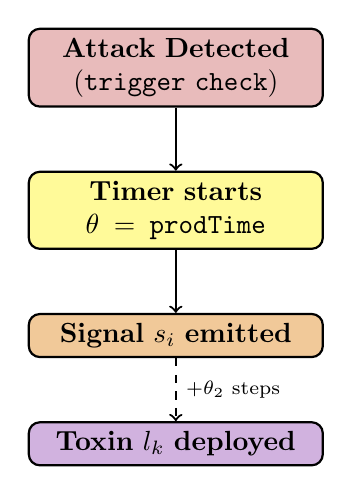
\begin{tikzpicture}[auto, thick]
            \node[rectangle, draw, fill=herbired!30, rounded corners, align=center, text width=3.5cm] (a) {\textbf{Attack Detected}\\(\texttt{trigger check})};
            \node[rectangle, draw, fill=yellow!40, rounded corners, align=center, text width=3.5cm, below=0.8cm of a] (t) {\textbf{Timer starts}\\\textbf{$\theta = \mathtt{prodTime}$}};
            \node[rectangle, draw, fill=signalorange!40, rounded corners, align=center, text width=3.5cm, below=0.8cm of t] (s) {\textbf{Signal $s_i$ emitted}};
            \node[rectangle, draw, fill=toxinpurple!30, rounded corners, align=center, text width=3.5cm, below=0.8cm of s] (x) {\textbf{Toxin $l_k$ deployed}};
            \draw[->] (a) -- (t);
            \draw[->] (t) -- (s);
            \draw[->, dashed] (s) -- node[right, font=\scriptsize]{+$\theta_2$ steps} (x);
        \end{tikzpicture}
        \end{center}
    \end{columns}
    \script{When a plant detects an attack, it cannot instantly deploy a complex toxin. It \textbf{requires theta time steps to synthesize} it -- note that production times are fully user-configurable parameters, not hardcoded constraints. During this countdown, the herbivore continues to eat the plant! This \textbf{creates a critical temporal vulnerability}. If a plant waits too long to trigger its defense, it may be dead before synthesis completes. This is precisely \textbf{why priming via VOC signals is so advantageous}: the neighbor's timer starts early, before the herbivore even arrives.}
    \qa{Do the timers $\theta$ break the standard step-wise transition of P systems?}{No, they can be formally mapped to standard P systems by using intermediate 'dummy' objects that rewrite step-by-step until $\theta$ is reached. The timer is simply a computational shortcut to avoid generating thousands of intermediate rules.}
\end{frame}

% =====================================================================
% Slide 8: The Formal System
% =====================================================================
\begin{frame}{The Formal System}
    We define the extended Tissue P System as:
    \begin{center}
        \Large $\Pi = (O,\; V_{n,n},\; E,\; \mathcal{R},\; t_{fin})$
    \end{center}
    \vspace{0.2cm}
    \begin{columns}[T, onlytextwidth]
        \column{0.5\textwidth}
        \begin{itemize}
            \item \textbf{$O$} (Object Alphabet):\\
            $\{e,\; s_1 \ldots s_{15},\; b_1 \ldots b_{15},\; l_1 \ldots l_{15},\; h_{m,\tau}\}$\\
            {\footnotesize energy $\cdot$ signals $\cdot$ bitter repellents $\cdot$ lethal toxins $\cdot$ herbivores}
            \item \textbf{$V_{\mu,\nu}$} (Cells):\\
            $(Q, q_0, w_0)_{\mu,\nu}$\\
            {\footnotesize allowed states $\cdot$ initial state $\cdot$ initial multiset}
            \item \textbf{$E$} (Edges): Mycorrhizal connections (adjacent pairs only)
        \end{itemize}

        \column{0.45\textwidth}
        \begin{itemize}
            \item \textbf{$\mathcal{R}$} (Rules): Timer-controlled, state-conditional multiset rewriting
            \item \textbf{$t_{fin}$}: Simulation termination condition
        \end{itemize}
        \vspace{0.4cm}
        \begin{block}{Cell State}
            $q \in \{\square,\; p_1, \ldots, p_{16}\}$\\
            $\square$: empty cell; $p_i$: occupied by species $i$
        \end{block}
    \end{columns}
    \script{To formally ground the simulation, \textbf{I modeled the environment as an extended Tissue P System}, denoted here as Pi. The \textbf{object alphabet O} comprises all physical and chemical entities: caloric energy, biochemical signals, repellents, toxins, and the herbivores themselves. \textbf{The cells V} represent spatial patches, tracking their own internal state -- empty or occupied -- and their starting multisets. The \textbf{edges E} represent the \textbf{underground Mycorrhizal connections} between adjacent patches. The \textbf{rules R} are the heart of the engine: they govern \textbf{state-conditional, timer-controlled multiset rewriting} to simulate complex biological interactions. Finally, the system runs until the \textbf{termination condition} is met.}
\end{frame}

% =====================================================================
% Slide 9: Key Rules
% =====================================================================
\begin{frame}{Formalizing Ecological Events as P System Rules}
    \vspace{0.1cm}
    \textbf{Photosynthesis} (energy gain per step $\theta=1$):
    \vspace{-0.1cm}
    $$[~]_{\mu,\nu}^{p_i} \xrightarrow{1} [\underbrace{e \ldots e}_{a}]_{\mu,\nu}^{p_i}$$

    \vspace{-0.1cm}
    \textbf{Herbivore Movement} (pathfinding toward nearest plant):
    \vspace{-0.1cm}
    $$[\underbrace{h_{m,\tau} \ldots}_{a}]_{\mu,\nu} \xrightarrow{\theta} [~]_{\mu,\nu}\;[\underbrace{h_{m,\tau} \ldots}_{a}]_{\alpha,\beta}$$

    \vspace{-0.1cm}
    \textbf{Signal Trigger} (emitter detects attack, sends $s_i$ via air, cost = \texttt{energyCosts}):
    \vspace{-0.1cm}
    $$[h_{m,\tau}^{(\geq k)},\; \underbrace{e \ldots e}_{c}]_{\mu,\nu}^{p_i} \xrightarrow{\theta_s} [s_i]_{radius} \;[\underbrace{e \ldots e}_{c-\delta}]_{\mu,\nu}^{p_i}$$

    \vspace{-0.1cm}
    {\small Where $k$ = \texttt{triggerCombination}, $\delta$ = \texttt{energyCosts}, $\theta_s$ = \texttt{prodTime}.}
    \script{These three rules capture the core ecological dynamics. \textbf{Photosynthesis adds energy} tokens each step for any membrane in plant state $p_i$. \textbf{Herbivore movement transfers} herbivore objects between membranes via BFS pathfinding. The \textbf{Signal Trigger is the heart of the model}: if a plant detects an attacker swarm of at least size $k$, it consumes delta energy tokens and emits the signal object $s_i$ across a specified radius, after a delay of theta steps.}
    \qa{Are these multiset rewriting rules cooperative?}{Yes, the ecological rules are highly cooperative. For example, the Signal Trigger rule requires the specific co-occurrence of herbivore objects ($h_m$) and energy objects ($e$) in the same membrane to produce a signal.}
\end{frame}

% =====================================================================
% Slide 10: Chemical Warfare Logic
% =====================================================================
\begin{frame}{Chemical Warfare: Trigger Combinations}
    \begin{columns}[T, onlytextwidth]
        \column{0.45\textwidth}
        \vspace{-0.5cm}
        \begin{center}
        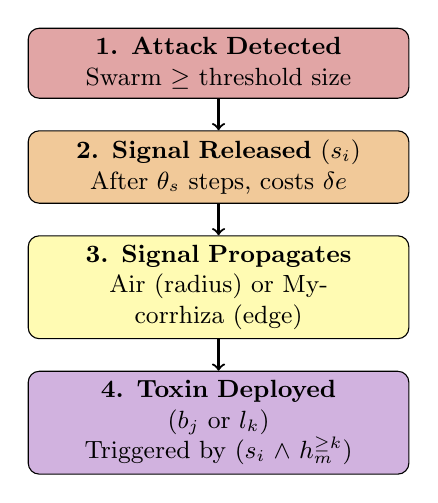
\begin{tikzpicture}[
            box/.style={rectangle, draw, rounded corners, text width=4.6cm, align=center, minimum height=0.75cm, font=\small}
        ]
            \node (n1) [box, fill=herbired!40] {\textbf{1. Attack Detected}\\ Swarm $\geq$ threshold size};
            \node (n2) [box, fill=signalorange!40, below=0.4cm of n1] {\textbf{2. Signal Released} ($s_i$)\\ After $\theta_s$ steps, costs $\delta e$};
            \node (n3) [box, fill=yellow!30, below=0.4cm of n2] {\textbf{3. Signal Propagates}\\ Air (radius) or Mycorrhiza (edge)};
            \node (n4) [box, fill=toxinpurple!30, below=0.4cm of n3] {\textbf{4. Toxin Deployed}\\ ($b_j$ or $l_k$)\\ Triggered by $(s_i \wedge h_m^{\geq k})$};
            \draw[->, thick] (n1) -- (n2);
            \draw[->, thick] (n2) -- (n3);
            \draw[->, thick] (n3) -- (n4);
        \end{tikzpicture}
        \end{center}

        \column{0.55\textwidth}
        \textbf{Trigger Combinations} are compound conditions:
        \vspace{0.2cm}
        \begin{itemize}\footnotesize
            \item \textbf{Signals} fire when \textit{any} specified enemy condition is met:\\
            {\footnotesize\texttt{trigger = [['e1', 2], ['e3', 1]]} \\ $\Rightarrow$ $\geq 2$ of $e_1$ \textbf{OR} $\geq 1$ of $e_3$}
            \item \textbf{Toxins} fire when a specific \textit{signal + enemy} condition is met:\\
            {\footnotesize\texttt{trigger = [['s1', 'e1', 1]]} \\ $\Rightarrow$ signal $s_1$ active AND $\geq 1$ of $e_1$}
        \end{itemize}
        \vspace{0.2cm}
        \begin{itemize}\footnotesize
            \item \textbf{Bitter repellents} ($b_j$, \texttt{deadly=False}): displace the herbivore cluster to a new path.
            \item \textbf{Lethal toxins} ($l_k$, \texttt{deadly=True}): reduce cluster size by \texttt{eliminationStrength}.
        \end{itemize}
    \end{columns}
    \script{The logic governing when defenses fire is highly configurable through \textbf{Trigger Combinations} -- these are compound Boolean conditions. A plant might only emit a signal if it detects both Enemy 1 AND Enemy 3 simultaneously. Once deployed, two types of substances exist: \textbf{Bitter repellents which displace} the herbivore cluster without killing it, forcing it to find a new path. And \textbf{lethal toxins which actively reduce} the cluster size by the configured elimination strength.}
    \qa{How is the environment $E$ formalized in this topology?}{The environment acts as the universal sink. When herbivores are eliminated by toxins, their corresponding objects are transferred to the environment. Airborne signals are also propagated through the environment topology to neighboring cells.}
\end{frame}

% =====================================================================
% Slide 11: Discrete Event Simulation Loop
% =====================================================================
\begin{frame}{The Discrete Event Execution Loop}
    Each simulation step executes a \textbf{fixed, ordered event sequence}:
    \vspace{0.3cm}
    \begin{center}
    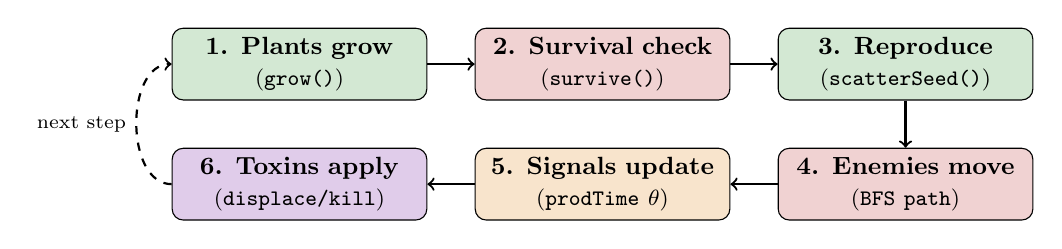
\begin{tikzpicture}[
        node distance=1.1cm and 1.5cm,
        box/.style={rectangle, draw, rounded corners, fill=blue!10, text width=3.0cm, text centered, minimum height=0.9cm, font=\small}
    ]
        \node[box, fill=plantgreen!20] (grow) {\textbf{1. Plants grow} \\ \footnotesize(\texttt{grow()})};
        \node[box, fill=herbired!20, right=0.6cm of grow] (surv) {\textbf{2. Survival check} \\ \footnotesize(\texttt{survive()})};
        \node[box, fill=plantgreen!20, right=0.6cm of surv] (repr) {\textbf{3. Reproduce} \\ \footnotesize(\texttt{scatterSeed()})};
        \node[box, fill=herbired!20, below=0.6cm of repr] (move) {\textbf{4. Enemies move} \\ \footnotesize(\texttt{BFS path})};
        \node[box, fill=signalorange!20, below=0.6cm of surv] (sig) {\textbf{5. Signals update} \\ \footnotesize(\texttt{prodTime} $\theta$)};
        \node[box, fill=toxinpurple!20, below=0.6cm of grow] (tox) {\textbf{6. Toxins apply} \\ \footnotesize(\texttt{displace/kill})};

        \draw[->, thick] (grow) -- (surv);
        \draw[->, thick] (surv) -- (repr);
        \draw[->, thick] (repr) -- (move);
        \draw[->, thick] (move) -- (sig);
        \draw[->, thick] (sig) -- (tox);
        \draw[->, thick, dashed] (tox.west) to[out=180, in=180] node[left, font=\scriptsize]{next step} (grow.west);
    \end{tikzpicture}
    \end{center}
    All steps execute for the \textit{entire grid} before advancing -- true discrete-event parallelism.
    \script{To prevent race conditions when simulating parallel biological processes on sequential hardware, we enforce a \textbf{strict discrete-event loop}. The \textbf{entire grid must complete one phase before advancing} to the next. This ordering matters: growth and survival run first to determine which cells are active, then reproduction, then movement, then signal updates based on where enemies now stand, and finally toxin application.}
    \qa{Can this model be simulated in standard tools like P-Lingua?}{Currently, our Python implementation acts as the simulator. Standard tools like P-Lingua lack built-in support for mapping spatial grid coordinates to visual frontends. However, the rule semantics themselves are fully compatible with P-Lingua syntax.}
\end{frame}

% =====================================================================
% Slide 12a: Software Architecture -- Stack
% =====================================================================
\begin{frame}{Software Architecture: Technology Stack}
    \begin{columns}[T, onlytextwidth]
        \column{0.5\textwidth}
        \vspace{0.2cm}
        \begin{itemize}
            \item \textbf{Language:} Python 3.12.5
            \item \textbf{Pattern:} Model-View-Controller (MVC)
            \item \textbf{Libraries:} NumPy, Matplotlib, Tkinter
        \end{itemize}
        \vspace{0.2cm}
        \centering
        {\small
        \begin{tabular}{@{}ll@{}}
            \toprule
            Layer & Key Classes \\
            \midrule
            \textbf{Model} & \texttt{Grid}, \texttt{Plant} \\
                           & \texttt{EnemyCluster} \\
                           & \texttt{Signal}, \texttt{Toxin} \\
                           & \texttt{Connection} \\
            \textbf{Controller} & \texttt{Simulation} \\
                                & \texttt{FileManager} \\
            \textbf{View} & \texttt{Gui}, \texttt{Diagrams} \\
            \bottomrule
        \end{tabular}
        }

        \column{0.45\textwidth}
        \vspace{-0.5cm}
        \begin{block}{Data Model}
            Each grid cell stores a tuple:\\[2pt]
            {\footnotesize\texttt{grid[x][y] = (Plant | None, [EnemyCluster, ...])}}
        \end{block}
        \vspace{0.1cm}
        \begin{block}{Persistence}
            {\small Scenarios serialized via \texttt{Exporter}/\texttt{Importer} (\texttt{pickle}).}
        \end{block}
        \vspace{0.1cm}
        \begin{block}{Diagrams}
            {\small Post-run time-series via \texttt{Diagrams.dataPlotter()}: energy, count, cluster size.}
        \end{block}
    \end{columns}
    \script{PlantProtectionSim is built in Python using a \textbf{strict Model-View-Controller architecture}. The \textbf{Model holds all logical state}: Grid, Plants, EnemyClusters, Signals, Toxins, and Connections. The \textbf{Controller drives the simulation loop} and handles file I/O via pickle serialization. The \textbf{View handles all rendering} in Tkinter and generates Matplotlib analytics charts after a run.}
    \qa{Why Python instead of C++?}{Python enables rapid prototyping, native Matplotlib integration for analytics, and straightforward pickle serialization for scenario persistence. Performance is well within requirements for our grid sizes.}
\end{frame}

% =====================================================================
% Slide 12b: Software Architecture -- MVC Flow
% =====================================================================
\begin{frame}{Software Architecture: MVC Interaction Flow}
    \begin{center}
    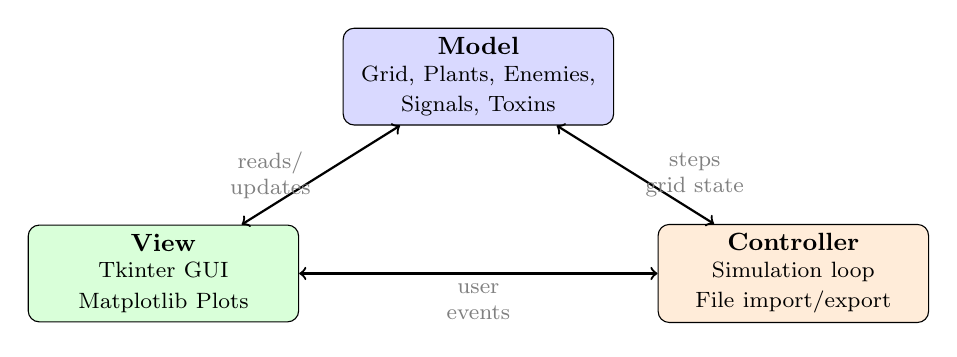
\begin{tikzpicture}[
        box/.style={rectangle, draw, rounded corners, text width=3.2cm, align=center, minimum height=1.1cm, font=\small},
        lbl/.style={font=\footnotesize, text=gray, align=center}
    ]
        \node[box, fill=blue!15] (m) at (0,0)
            {\textbf{Model}\\\footnotesize Grid, Plants, Enemies,\\Signals, Toxins};
        \node[box, fill=green!15] (v) at (-4,-2.5)
            {\textbf{View}\\\footnotesize Tkinter GUI\\Matplotlib Plots};
        \node[box, fill=orange!15] (c) at (4,-2.5)
            {\textbf{Controller}\\\footnotesize Simulation loop\\File import/export};

        \draw[<->, thick] (m) -- node[lbl, left]{reads/\\updates} (v);
        \draw[<->, thick] (m) -- node[lbl, right]{steps\\grid state} (c);
        \draw[<->, thick] (v) -- node[lbl, below]{user\\events} (c);
    \end{tikzpicture}
    \end{center}
    \vspace{0.2cm}
    \begin{center}
    {\small The GUI triggers the \texttt{Simulation.runStep()} loop; the View reads the grid state after each step to refresh the canvas.}
    \end{center}
    \script{The \textbf{MVC decoupling is key}. The Controller steps the Model forward. The \textbf{View is entirely passive} -- it simply reads the grid state at the end of each step and redraws the canvas. This clean separation means we could easily \textbf{replace the Tkinter GUI with a headless batch-processing runner} for large-scale parameter sweeps without touching the model logic.}
    \qa{Is the GUI updating synchronously?}{Yes, the simulation loop yields briefly after each step to allow the Tkinter canvas to refresh, giving the user real-time visual feedback.}
\end{frame}

% =====================================================================
% Slide 13: Biological Motivation: Plant Survival
% =====================================================================
\begin{frame}{Configurable Simulation Grid}
    \begin{columns}[T, onlytextwidth]
        \column{0.5\textwidth}
        \vspace{0.1cm}
        \textbf{Fully parameterizable configuration}:
        \vspace{0.1cm}
        \begin{itemize}\footnotesize
            \item \textbf{Plants:}\\ \texttt{initEnergy}, \texttt{growthRateEnergy}, \texttt{minEnergy}, \texttt{reproductionInterval}, \texttt{minDist}/\texttt{maxDist}
            \item \textbf{Herbivores:}\\ \texttt{num}, \texttt{speed}, \texttt{eatingSpeed}, \texttt{eatVictory}
            \item \textbf{Substances:}\\ \texttt{spreadType}, \texttt{prodTime}, \texttt{deadly}, \texttt{eliminationStrength}
            \item \textbf{Trigger:}\\ Compound species-specific conditions
        \end{itemize}

        \column{0.45\textwidth}
        \begin{center}
            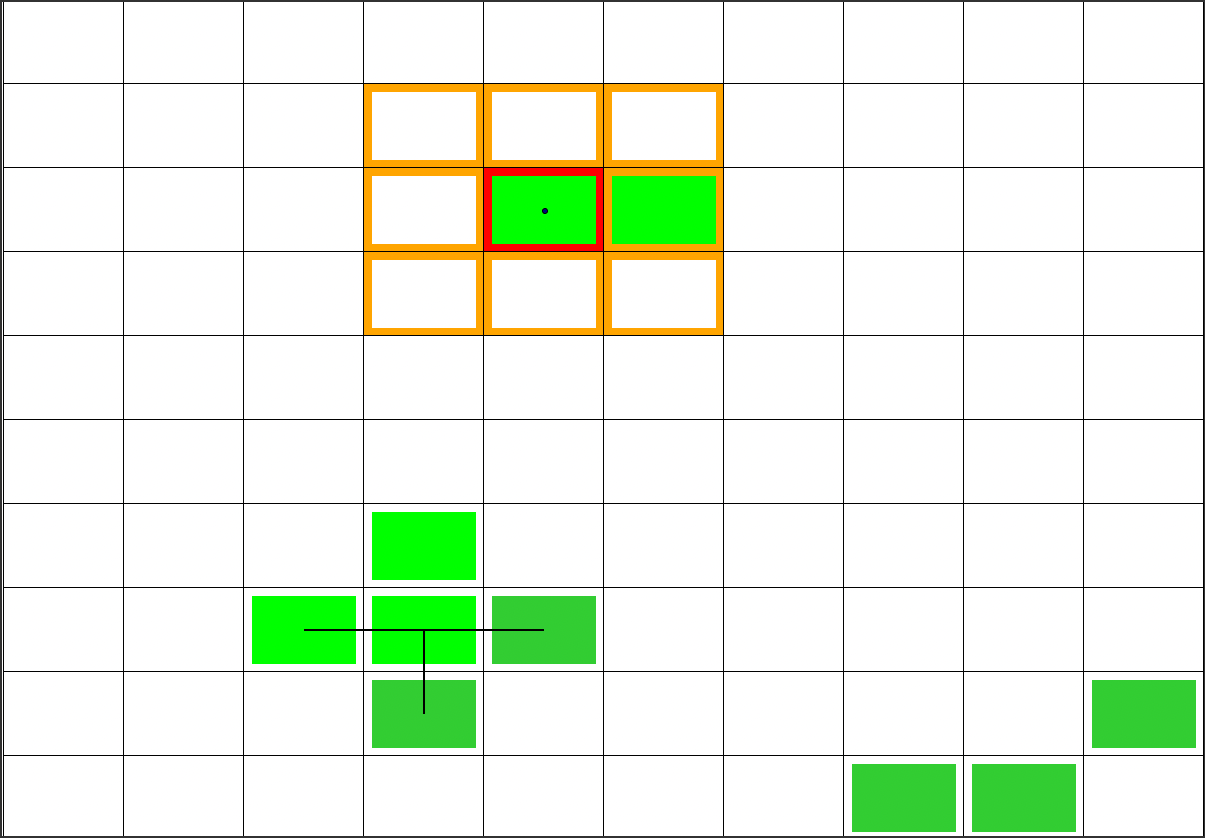
\includegraphics[width=0.92\textwidth, keepaspectratio]{figures/gui.png}
        \end{center}
    \end{columns}
    \script{PlantProtectionSim acts as a \textbf{highly configurable digital terrarium}. \textbf{Every agent property is tweakable} through the GUI. Plants: initial energy, growth rate, minimum energy threshold, reproduction interval, and dispersal distance. Herbivores: starting count, movement speed, eating speed, and victory energy gain. Substances: spread type, synthesis delay, lethality, and elimination strength. Trigger logic is fully compound and species-specific.}
    \qa{Can biological datasets be loaded into this?}{Currently parameters are synthetic and abstract. However the tool is designed so that if biologists quantify exact energy ratios or eating rates, they can be directly plugged into the configuration.}
\end{frame}

% =====================================================================
% Slide 14: Grid Visualization
% =====================================================================
\begin{frame}{Grid Cell Visual Grammar}
    \begin{columns}[T, onlytextwidth]
        \column{0.55\textwidth}
        Each cell encodes visual information in distinct \textbf{spatial layers}:
        \begin{itemize}\footnotesize
            \item \textbf{Inner square (Plant Domain):}\\
            Color saturation reflects energy level. Species identity encoded by hue ($p_1 =$ green, $p_2 =$ teal, \ldots). Empty cell = gray.
            \item \textbf{Center dot (Herbivores):}\\
            Binary representation: a single black dot in the center indicates herbivore presence. Detailed count information is hidden in a mouseover tooltip.
            \item \textbf{Outer border (Substance Domain):}\\
            Yellow/orange border = active signal.\\
            Red border = active toxin.
        \end{itemize}
        \vspace{0.1cm}
        This dual-layer grammar makes multi-species dynamics \textbf{visually readable at a glance}.

        \column{0.45\textwidth}
        \begin{center}
        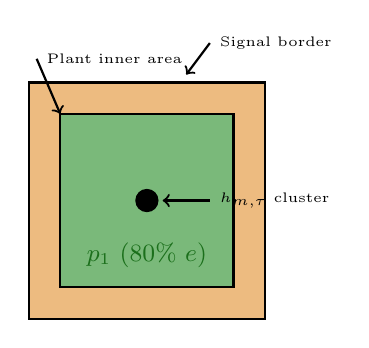
\begin{tikzpicture}[scale=1.0]
            % Cell with plant + herbivore
            \draw[fill=signalorange!50, thick] (0,0) rectangle (3,3);
            \draw[fill=plantgreen!60, thick] (0.4,0.4) rectangle (2.6,2.6);
            \node[font=\small, plantgreen!80!black] at (1.5, 0.8) {$p_1$ (80\% $e$)};
            % herbivore dot centered
            \filldraw[black] (1.5, 1.5) circle (4pt);
            % labels
            \draw[<-, thick] (1.7, 1.5) -- (2.3, 1.5) node[right, font=\tiny]{$h_{m,\tau}$ cluster};
            \draw[<-, thick] (2.0, 3.1) -- (2.3, 3.5) node[right, font=\tiny]{Signal border};
            \draw[<-, thick] (0.4, 2.6) -- (0.1, 3.3) node[right, font=\tiny]{Plant inner area};
        \end{tikzpicture}
        \end{center}
    \end{columns}
    \script{To make multi-species dynamics readable at a glance, we designed a \textbf{three-layer visual grammar}. The \textbf{inner square is the plant domain}: color hue encodes species, saturation encodes energy level. A \textbf{single black dot in the center signals herbivore presence} in a binary fashion -- detailed swarm counts are available on mouseover. The \textbf{outer border is the substance domain}: yellow or orange means an active VOC signal, red means an active toxin.}
    \qa{Why binary for herbivores and not showing the exact count?}{When swarms reach large numbers, drawing individual dots creates a visual mess. A binary indicator keeps spatial dynamics readable, while preserving exact data interactively in the tooltip.}
\end{frame}

% =====================================================================
% Slide 15: Case Study Setup
% =====================================================================
\begin{frame}{Case Study: 15×15 Biotope}
    \begin{columns}[T, onlytextwidth]
        \column{0.52\textwidth}
        {\small\textbf{Setup:} $15\times15 = 225$ cells, 2 plant species, 2 herbivore species, 3 substances.}
        \vspace{0.15cm}
        \begin{center}
        {\small\begin{tabular}{@{}lll@{}}
            \toprule
            Agent & Strategy & Key Trait \\
            \midrule
            $p_1$ & Repelling & Local dispersal \\
            $p_2$ & Lethal & Wide dispersal \\
            $h_1$ & Fast eater & High \texttt{eatVictory} \\
            $h_2$ & Slow, large & High \texttt{num} \\
            \bottomrule
        \end{tabular}
        }
        \end{center}
        \vspace{0.1cm}
        \begin{itemize}\footnotesize
            \item $s_1$ (air): fires when $h_1 \geq 10 \vee h_2 \geq 30$
            \item $b_1$ (repel): triggered by $s_1 \wedge (h_1 \geq 20 \vee h_2 \geq 40)$
            \item $l_1$ (lethal): triggered by $s_1 \wedge (h_1 \geq 40 \vee h_2 \geq 15)$

        \end{itemize}

        \column{0.48\textwidth}
        \begin{center}
            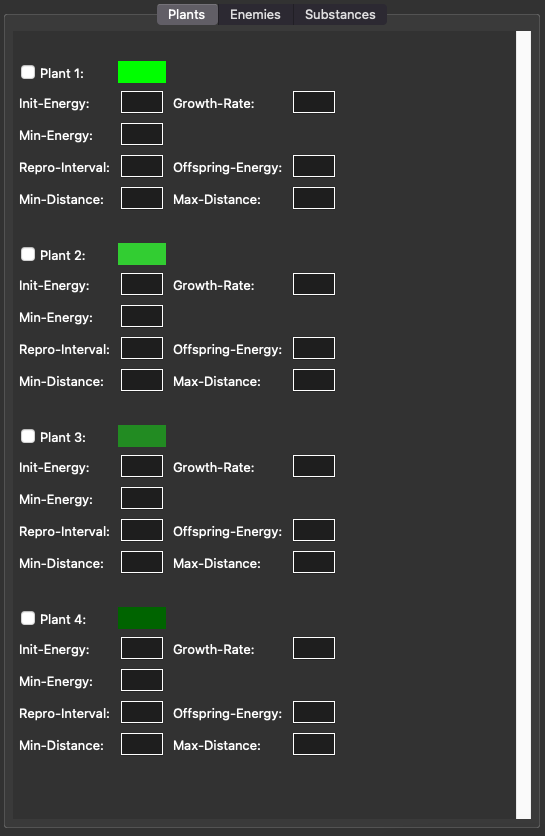
\includegraphics[width=\textwidth, height=0.70\textheight, keepaspectratio]{figures/grid.png}
        \end{center}
    \end{columns}
    \script{In our concrete case study we run a \textbf{15 by 15 grid} with 225 cells. We pit \textbf{two plant species against two herbivore species}. Plant 1 is a local disperser using bitter repellents; Plant 2 is a wide disperser using lethal toxins. Herbivore 1 is a fast eater; Herbivore 2 is slow but comes in large numbers. The trigger logic on the left shows how the \textbf{defensive cascade is chained}: signal fires on co-occurrence, repellent fires on signal plus enemy, toxin fires on a more extreme compound condition.}

\end{frame}

% =====================================================================
% Slide 16: Empirical Results
% =====================================================================
\begin{frame}{Empirical Results: Emergent Population Dynamics}
    \begin{columns}[T, onlytextwidth]
        \column{0.42\textwidth}
        \vspace{0.2cm}
        \begin{itemize}
            \item After an initial transient, the system enters a \textbf{persistent oscillatory regime}.
            \item \textbf{Lotka-Volterra pattern} emerges organically from the discrete rules -- no differential equations needed.
            \item Spatial constraints drive the oscillations: herbivores must physically travel to find plants, giving populations time to recover.
            \item \textbf{Coexistence} of two plant and two herbivore species is maintained.
        \end{itemize}

        \column{0.58\textwidth}
        \begin{center}
            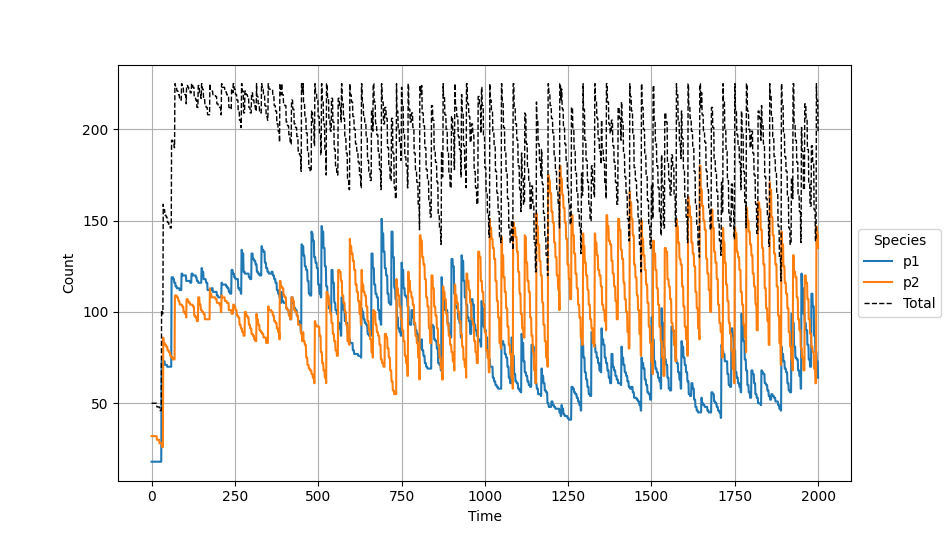
\includegraphics[width=\textwidth]{figures/plot.png}
        \end{center}
    \end{columns}
    \script{When we run this case study, something remarkable emerges. Without writing a single differential equation, the system naturally falls into a \textbf{persistent oscillatory regime} -- a textbook \textbf{Lotka-Volterra predator-prey curve}. This emerges entirely from discrete spatial constraints: herbivores eat plants, their population spikes, food runs scarce and they must travel, giving plants time to recover. This \textbf{spatial delay is the mechanism that maintains coexistence} of all four species.}

\end{frame}

% =====================================================================
% Slide 17: Simulation Demo (video)
% =====================================================================
\begin{frame}{Live Simulation: Case Study Run}
    \vspace{-0.2cm}
    \begin{center}
        % \href{run:...} opens the video in the OS default player.
        % Works in Acrobat, Okular, Evince, and all PDF readers that
        % pass run: links to the system. The path is relative to the PDF.
        \href{run:misc/zeitraffer-fallstudie-lucas.mp4}{%
            \fcolorbox{blue!50}{black!88}{%
                \begin{minipage}[c][0.72\textheight][c]{0.94\textwidth}
                    \centering
                    {\color{white}\Large\textbf{\textit{PlantProtectionSim} --- Case Study Run}}\\
                    \vspace{0.35cm}
                    {\color{white!75}\normalsize 15$\times$15 biotope $\cdot$ 2 plant species $\cdot$ 2 herbivore species}\\
                    {\color{white!75}\normalsize $\sim$141 seconds time-lapse}\\
                    \vspace{0.45cm}
                    {\color{signalorange}\fontsize{40}{40}\selectfont$\blacktriangleright$}\\
                    \vspace{0.35cm}
                    {\color{white!70}\small\textbf{Click to open in system video player}}\\[0.15cm]
                    {\color{white!45}\scriptsize Works in Okular, Evince, Acrobat, VLC and all PDF readers}
                \end{minipage}%
            }%
        }\\[0.15cm]
        {\tiny\color{gray} \texttt{misc/zeitraffer-fallstudie-lucas.mp4} \quad H.264/AAC}
    \end{center}
    \script{\textbf{This is a live recording of the case study run} we just described formally. The video is a 2-minute time-lapse of the 15 by 15 grid. Watch the \textbf{colour waves spreading} -- those are VOC signals propagating to neighbouring cells. \textbf{Red-bordered cells are under attack}. Notice how the \textbf{oscillatory rhythm} we saw in the population plot manifests spatially: herbivore clusters sweep across the grid, plants recover in their wake, then the cycle repeats. \textbf{The key message is emergence}: no single rule encodes a Lotka-Volterra cycle -- it arises purely from local multiset rewriting.}
\end{frame}

% =====================================================================
% Slide 18: Conclusions
% =====================================================================
\begin{frame}{Conclusions}
    \begin{columns}[T, onlytextwidth]
        \column{0.65\textwidth}
        \textbf{Contributions}
        \begin{itemize}\footnotesize
            \item Extended Tissue P Systems with \textbf{energy tokens}, \textbf{membrane states}, and \textbf{countdown timers} to faithfully model ecological dynamics.
            % \item Visual, fully configurable discrete event simulator -- \textit{PlantProtectionSim}.
            \item Emergent Lotka-Volterra dynamics from purely rule-based P system computation.
        \end{itemize}
        \vspace{0.15cm}
        \textbf{Towards Production-Scale Simulation}
        \begin{itemize}\footnotesize
            \item PlantProtectionSim demonstrates the \textbf{formal validity} of the extended Tissue P system model.
            \item The next step: translate these P system semantics into a \textbf{massively parallel, continuous-field engine} capable of multi-km$^2$ biotopes with millions of entities.
            \item \textbf{PHIDS} (Plant-Herbivore Interaction \& Defense Simulator) realizes precisely this -- and goes further by coupling discrete entity dynamics with continuous Reaction-Diffusion PDEs for airborne VOC fields.
        \end{itemize}

        \column{0.35\textwidth}
        \begin{center}
        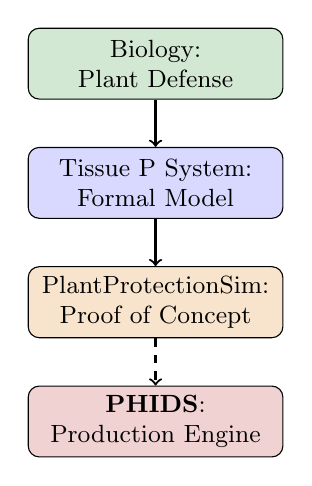
\begin{tikzpicture}[scale=0.8,
            box/.style={rectangle, draw, rounded corners, fill=gray!10, text width=3.0cm, align=center, minimum height=0.9cm, font=\small}
        ]
            \node[box, fill=plantgreen!20] (bio) {Biology:\\Plant Defense};
            \node[box, fill=blue!15, below=0.6cm of bio] (p) {Tissue P System:\\Formal Model};
            \node[box, fill=signalorange!20, below=0.6cm of p] (sim) {PlantProtectionSim:\\Proof of Concept};
            \node[box, fill=herbired!20, below=0.6cm of sim] (phids) {\textbf{PHIDS}:\\Production Engine};
            \draw[->, thick] (bio) -- (p);
            \draw[->, thick] (p) -- (sim);
            \draw[->, thick, dashed] (sim) -- (phids);
        \end{tikzpicture}
        \end{center}
    \end{columns}
    \script{In conclusion: we \textbf{extended Tissue P Systems} with energy tokens, membrane states, and countdown timers to faithfully represent ecological dynamics. We built PlantProtectionSim as a visual, fully configurable tool that demonstrates these formal dynamics. Our empirical results show \textbf{emergent Lotka-Volterra behavior} from purely rule-based computation. But this presentation is actually the \textbf{beginning of a larger story}. PlantProtectionSim is the formal proof-of-concept. The natural next evolution is a \textbf{production-grade engine that preserves the same mathematical semantics} but operates at an entirely different scale -- and that engine is called PHIDS.}
    \qa{How does PHIDS relate formally to the P system model we presented?}{PHIDS preserves the core membrane semantics -- each grid cell remains an independent state-carrying compartment with multiset-like component arrays. The key architectural advance is parallelizing all rewriting rules across the full spatial grid simultaneously via branchless array operations, replacing Python object dispatch with vectorized field mathematics.}
\end{frame}


% =====================================================================
% Slide: Thank You
% =====================================================================
\begin{frame}[plain]
    \begin{center}
        \vspace{1.5cm}
        {\Huge \textbf{Thank You!}}
        \vspace{0.8cm}

        {\Large Questions?}
        \vspace{1.0cm}

        \begin{tabular}{ll}
            \textbf{Author:} & Benjamin Förster \\
            \textbf{Conference:} & ICMC 2026 -- Seville (Spain) \\
            \textbf{Paper:} & \textit{PlantProtectionSim} -- Tissue P System Application \\
        \end{tabular}
    \end{center}
    \script{\textbf{Thank you for your attention}. I am happy to answer any questions. If needed, I can navigate back to any specific slide.}
\end{frame}

% =====================================================================
% PHIDS Annex 1: Technical Architecture & Development Profile
% =====================================================================
\begin{frame}{PHIDS: Architecture \& Development Profile}
    \begin{columns}[T, onlytextwidth]
        \column{0.55\textwidth}
        \textbf{Project Scale (6 Months, 1 Dev)}
        \begin{itemize}\footnotesize
            \item \textbf{Lines of Code:} $\sim$74,000 total ($\sim$54k Python).
            \item \textbf{Complexity:} 3,379 SCC metric across 461 files.
            \item \textbf{Organic Estimate:} \$1.6M cost, 16 months for a 9-person team.
        \end{itemize}
        \vspace{0.2cm}
        \textbf{Core Architecture}
        \begin{itemize}\footnotesize
            \item \textbf{Parallel In-Memory Execution:} Data-Oriented ECS (arrays over objects) for maximum throughput.
            \item \textbf{Just-In-Time (JIT) Compilation:} Pre-compiled numerical hot-paths eliminate Python bottlenecks.
            \item \textbf{O(1) Spatial Hashing:} Constant-time grid lookups for rapid agent interaction and collision.
            \item \textbf{Double Buffering:} Strict read/write state separation ensures deterministic reproducibility.
        \end{itemize}

        \column{0.45\textwidth}
        \vspace{-0.95cm}
        \begin{center}
            
\includegraphics[width=0.70\textwidth, keepaspectratio]{figures/PHIDS/Logo_cropped.png}\\[0.1cm]
            \begin{tabular}{@{}c@{\hskip 0.4cm}c@{}}
                \vspace{-0.5cm}
                \qrcode[height=1.8cm]{https://github.com/foersben/PHIDS\#readme} & \qrcode[height=1.8cm]{https://foersben.github.io/PHIDS/} \\
                \vspace{0.0cm}\\
                \footnotesize\textbf{Repository} & \footnotesize\textbf{Docs}
            \end{tabular}
        \end{center}
    \end{columns}
    \script{In this annex, \textbf{I want to showcase PHIDS}: the next-generation simulation engine \textbf{I developed from scratch in just six months}. By architecting a \textbf{Data-Oriented Entity-Component-System} and implementing \textbf{Just-In-Time compilation}, \textbf{I achieved massive parallelism}. In classic ABMs like \textbf{NetLogo or AnyLogic}, finding neighbors requires slow $O(N)$ object iteration or complex trees. Because I built strict memory foundations like \textbf{O(1) spatial hashing} -- turning spatial queries into instant array lookups -- and \textbf{subnormal float clamping}, the engine achieves massive throughput. And by enforcing \textbf{deterministic double-buffering}, it avoids race conditions entirely, guaranteeing mathematical reproducibility even during parallel batch processing. This technological leap is the core of our EXIST market strategy: we aim to acquire \textbf{30 Pro and 5 Enterprise customers} by leveraging this massive batch processing on cloud servers, streaming telemetry directly to disk with \textbf{zero UI overhead} for industrial R\&D.}
\end{frame}

% =====================================================================
% PHIDS Annex 2: Core Simulation Concepts
% =====================================================================
\begin{frame}{PHIDS: Core Simulation Concepts}
    \begin{itemize}
        \item \textbf{Biological Actors (Swarms \& Flora):} Herbivore swarms and plants act as discrete entities driving population dynamics through foraging and swarm mitosis. Plants follow complex developmental lifecycles governed by two decoupled state properties: \textit{caloric energy} and \textit{structural mass}.
        \item \textbf{Reaction-Diffusion Dynamics:} Airborne Volatile Organic Compounds (VOCs) form continuous scalar fields that decay and diffuse, priming downwind flora defenses.
        \item \textbf{Flow Fields \& Advection:} Gaussian plumes explicitly model wind drift, providing directional signal transport across the biotope.
        \item \textbf{Chemotactic Foraging:} Herbivores sample local chemical gradients rather than having omniscient knowledge, abandoning patches based on the Marginal Value Theorem.
        \item \textbf{Mycorrhizal Symbiosis:} Fungal networks enable instantaneous underground signal propagation, bypassing atmospheric delays for a metabolic cost.
    \end{itemize}
    \script{\textbf{I designed the core} of PHIDS around discrete biological actors driven by strict \textbf{metabolic attrition}. \textbf{I implemented Reaction-Diffusion dynamics} to explicitly simulate airborne signals drifting via Gaussian plumes. The herbivores here are not omniscient; \textbf{I built them to navigate chemotactically} and abandon food patches dynamically based on the \textbf{Marginal Value Theorem}. Furthermore, \textbf{I integrated underground fungal networks} to allow rapid signal propagation in exchange for a metabolic tax.}
\end{frame}

% =====================================================================
% PHIDS Annex 3: EEDSE \& Empirical Foundations
% =====================================================================
\begin{frame}{PHIDS: EEDSE \& Empirical Foundations}
    \begin{itemize}
        \item \textbf{Evolutionary Encapsulated Design Space Exploration (EEDSE):} Finding a stable Lotka-Volterra coexistence via multi-objective genetic algorithms (e.g., NSGA-II/III). Thousands of parameter configurations are evaluated.
        \item \textbf{Bio-Databases:} The simulation operates on empirically calibrated parameters. Traits are anchored directly to real biological databases:
        \begin{itemize}\footnotesize
            \item \textbf{TRY \& Dr. Duke's:} Structural biomass, growth rates, and phytochemical profiles.
            \item \textbf{PanTHERIA:} Mammalian baseline metabolic upkeep and caloric demands.
            \item \textbf{Pherobase \& NIST:} Chemical diffusivity constants and VOC properties.
            \item \textbf{GloBI \& GBIF:} Trophic interaction networks and spatial occurrence data.
            \item \textbf{ToxValDB:} Empirical toxicity thresholds for defensive compounds.
        \end{itemize}
        \item \textbf{Data Imputation (k-NN / k-Means):} Missing traits in the databases are systematically reconstructed via phylogenetic k-Nearest Neighbors and k-Means clustering to ensure complete parameter sets.
        \item \textbf{Thermodynamic Pre-Pruning:} EEDSE analytically rejects infeasible configurations before simulation (e.g., if total plant growth cannot sustain herbivore metabolism).
    \end{itemize}
    \script{To guarantee \textbf{scientific validity}, \textbf{I engineered an Evolutionary Design Space Exploration} framework. \textbf{I use genetic algorithms} to discover stable coexistences across thousands of parameter sets. Crucially, \textbf{I anchored every single trait to real-world empirical databases} like TRY and PanTHERIA. Where data was missing, \textbf{I implemented k-NN and k-Means clustering} to systematically reconstruct it. Finally, my \textbf{thermodynamic pre-pruning} analytically rejects impossible configurations \textbf{before they ever waste CPU time}.}
\end{frame}

% =====================================================================
% PHIDS Annex 2: Live Simulation View
% =====================================================================
\begin{frame}[plain]
    \begin{center}
        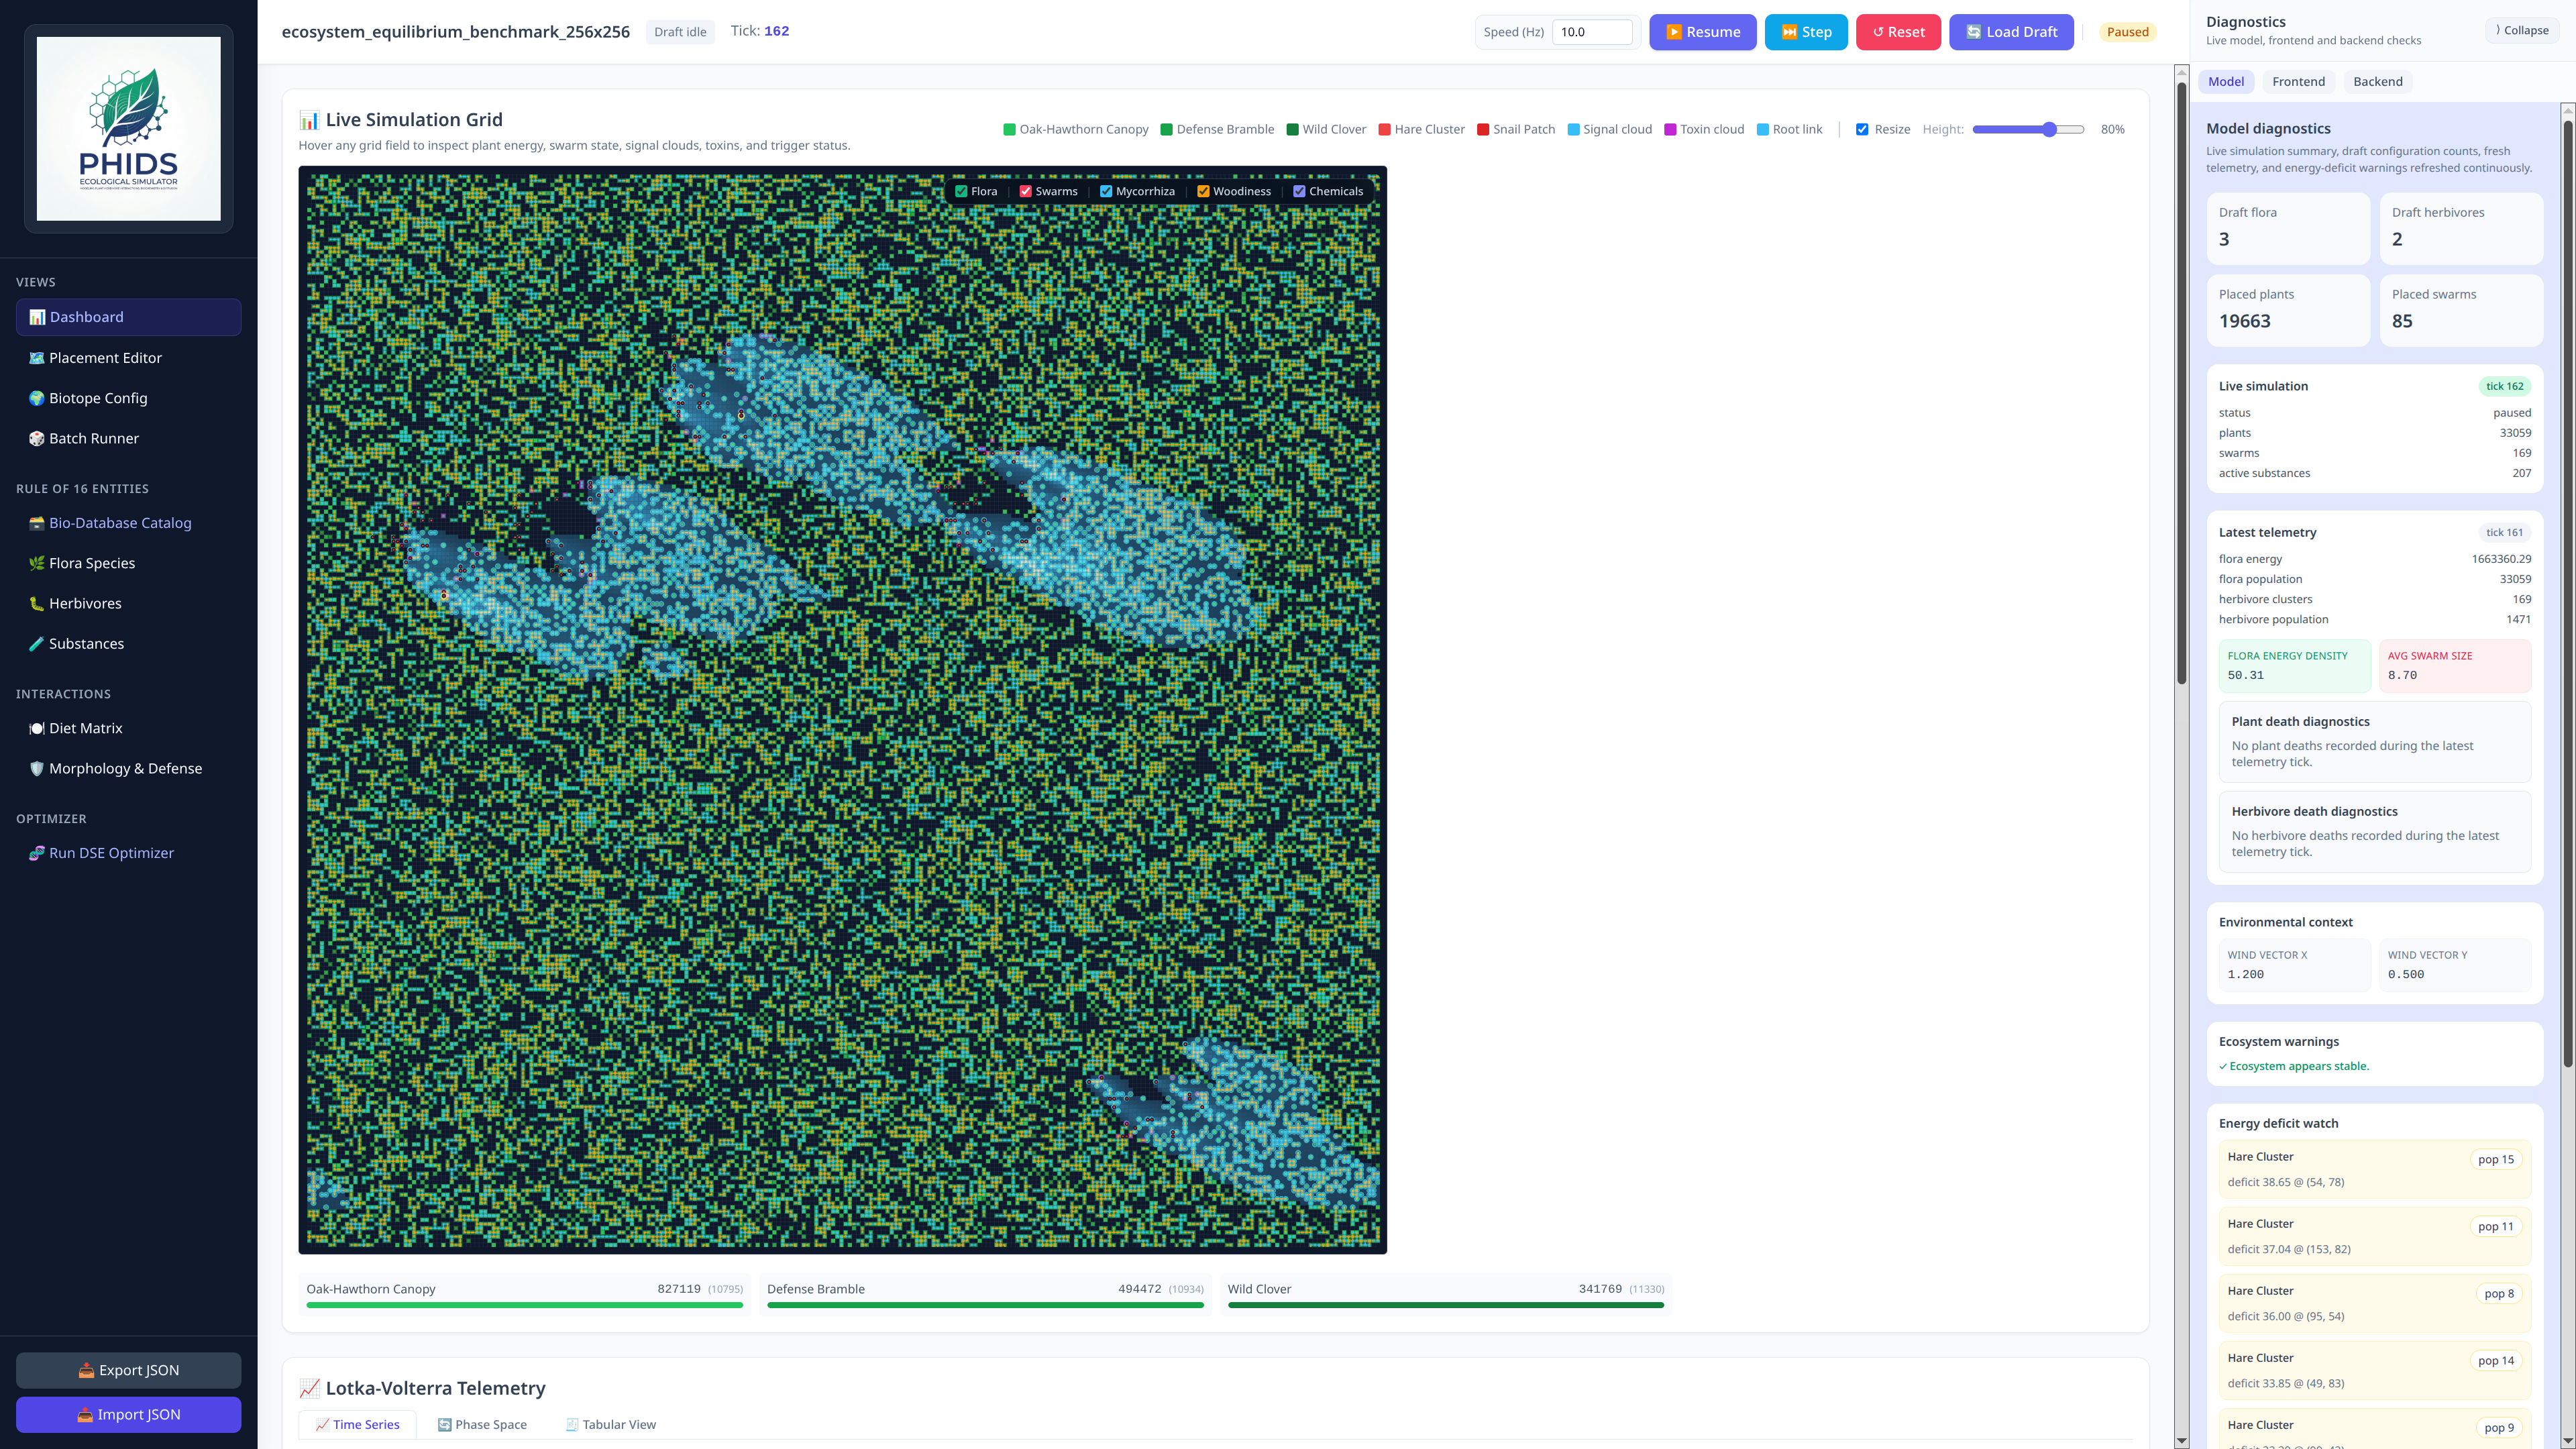
\includegraphics[width=\textwidth, height=0.98\textheight, keepaspectratio]{figures/PHIDS/PHIDS_Live.png}
    \end{center}
    \script{\textbf{Here is a glimpse into the live simulation view I built}. Even though I aggressively optimized the engine for headless batch processing, \textbf{I also developed a fully responsive UI} to allow for \textbf{real-time monitoring} of population dynamics, spatial flow fields, and continuous chemical gradients.}
\end{frame}

% =====================================================================
% PHIDS Annex 3: Cell Diagnostics
% =====================================================================
\begin{frame}[plain]
    \begin{center}
        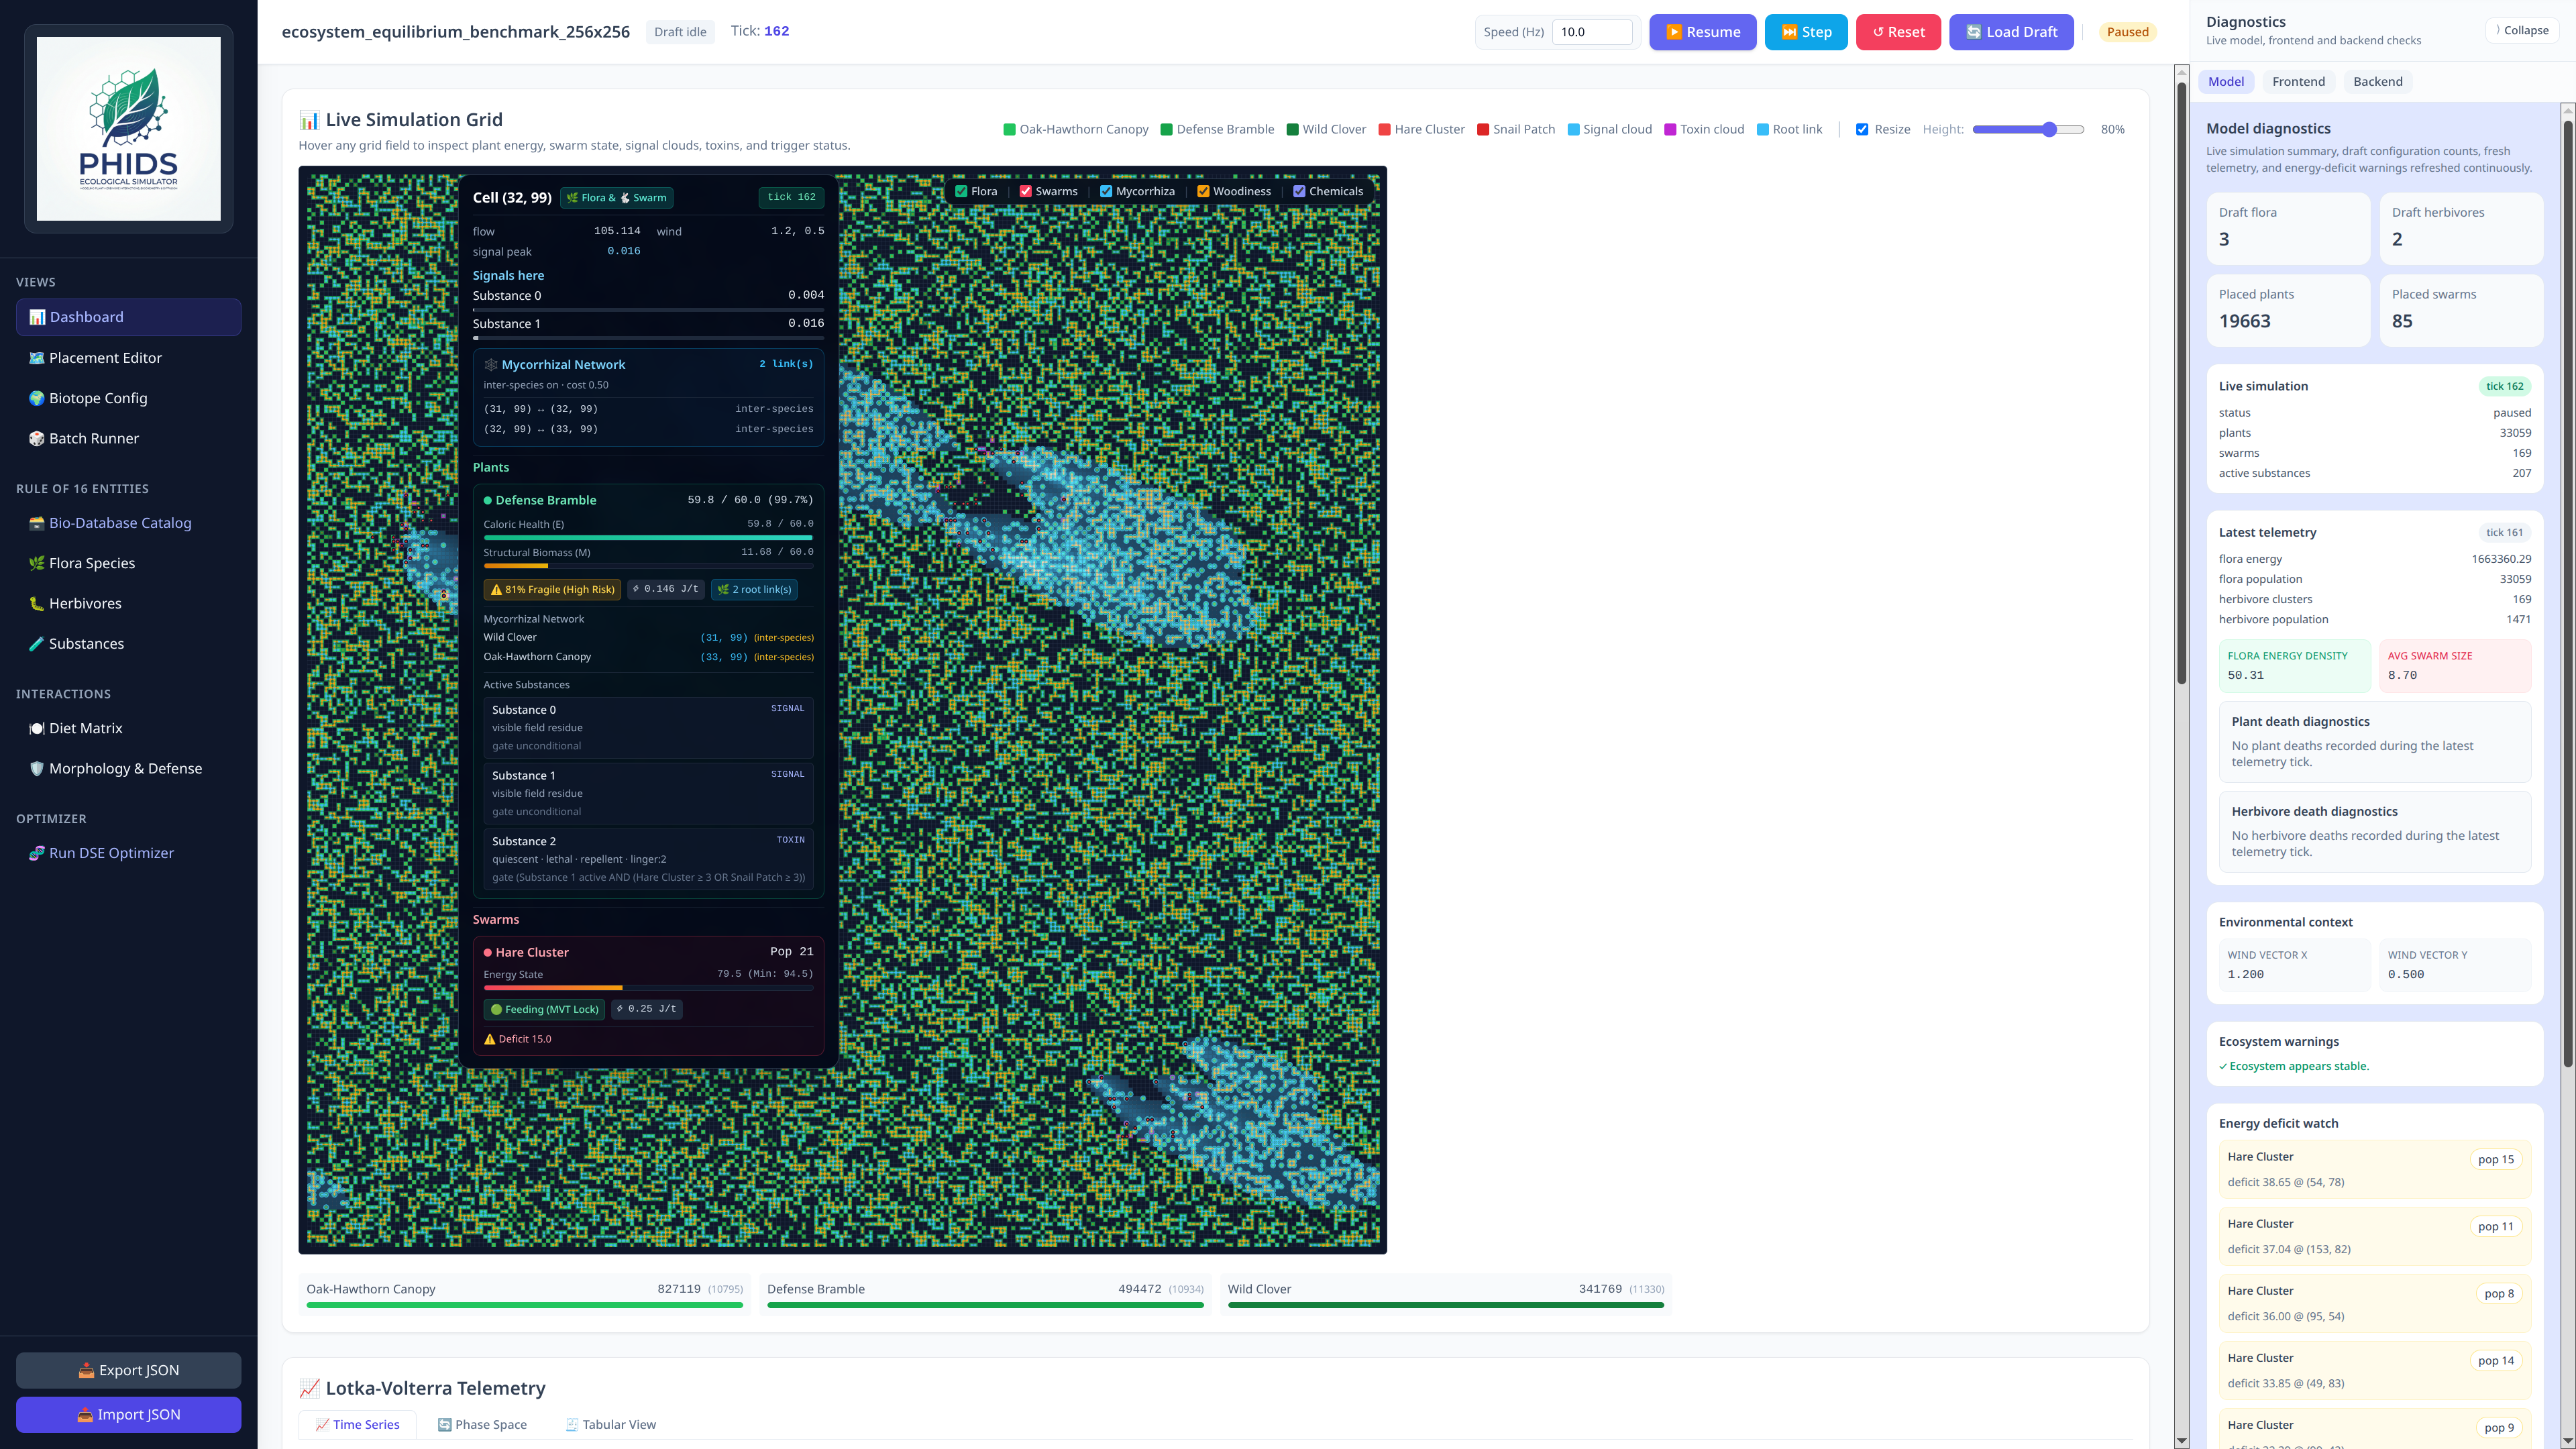
\includegraphics[width=\textwidth, height=0.98\textheight, keepaspectratio]{figures/PHIDS/PHIDS_tooltip.png}
    \end{center}
    \script{Finally, \textbf{I implemented detailed cell diagnostics}. Every single grid cell and entity can be \textbf{inspected during runtime}. This allows us to track metabolic states, localized chemical concentrations, and environmental limits -- \textbf{perfectly bridging the gap} between empirical data and visual simulation.}
\end{frame}

\end{document}
